\chapter{Leviticus 12}

\begin{figure}
  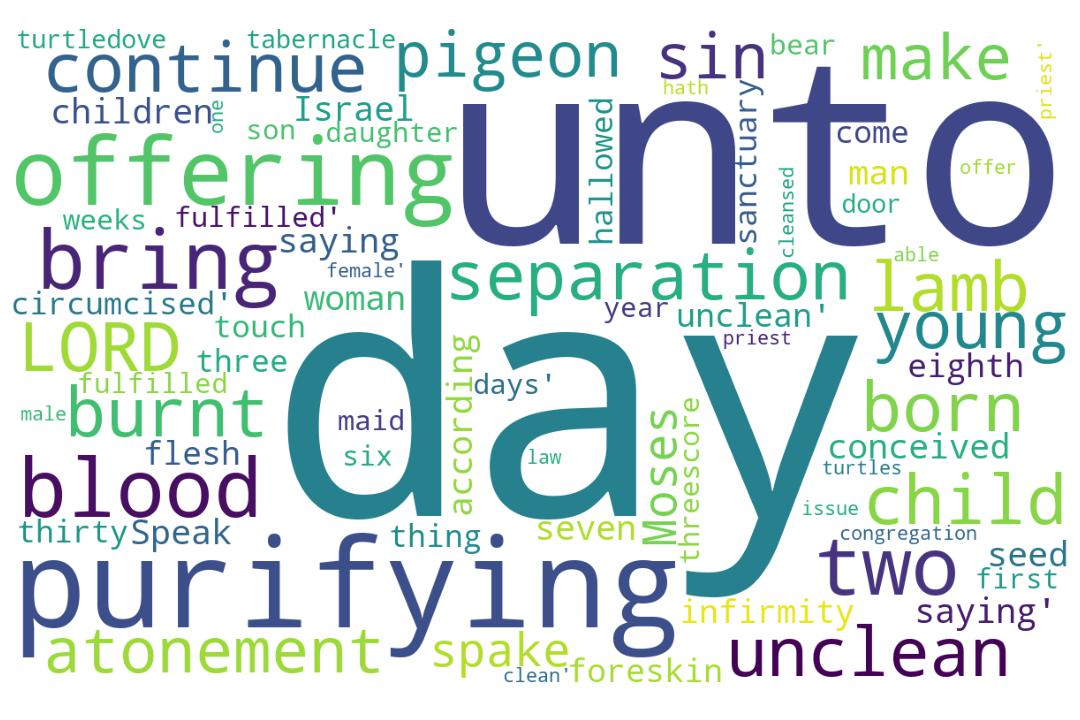
\includegraphics[width=\linewidth]{03OT-Leviticus/Leviticus12-WordCloud.jpg}
  \caption{Leviticus 12 Word Cloud}
  \label{fig:Leviticus 12 word Cloud}
\end{figure}

\marginpar{\scriptsize \centering \fcolorbox{bone}{lime}{\textbf{A POSTPARTUM BATH}}\\ (Leviticus 12:1--8) 
\begin{compactenum}[I.][8]
    \item \textbf{Time Periods} 
    \begin{compactenum}[A.][7]
		\item seven days  \index[scripture]{Leviticus!Lev 12:02} (Lev 12:2)
		\item eighth day \index[scripture]{Leviticus!Lev 12:03} (Lev 12:3)
		\item three and thirty days \index[scripture]{Leviticus!Lev 12:04} (Lev 12:4)
		\item two weeks \index[scripture]{Leviticus!Lev 12:05} (Lev 12:5)
		\item threescore and six days \index[scripture]{Leviticus!Lev 12:05} (Lev 12:5)
		\item first year \index[scripture]{Leviticus!Lev 12:06} (Lev 12:6)
    \end{compactenum}
    \item A \textbf{Telling Proclamation} \index[scripture]{Leviticus!Lev 12:02} (Lev 12:2)
    \item \textbf{Total Purification}  \index[scripture]{Leviticus!Lev 12:04} (Lev 12:4)
    \item \textbf{Verboten Place}  \index[scripture]{Leviticus!Lev 12:04} (Lev 12:4)
    \item \textbf{Trusted Priest} \index[scripture]{Leviticus!Lev 12:06} (Lev 12:6)
    \item \textbf{Turtles \& Pigeons}  \index[scripture]{Leviticus!Lev 12:08} (Lev 12:8)
\end{compactenum} 
}

%%%%%%%%%%%%%%%%%%%%%%%%%%%%%%%%%%
%%%%%%%%%%%%%%%%%%%%%%%%%%%%%%%%%%
\footnote{\textcolor[cmyk]{0.99998,1,0,0}{\hyperlink{TOC}{Return to end of Table of Contents.}}}\footnote{\href{https://audiobible.com/bible/leviticus_12.html}{\textcolor[cmyk]{0.99998,1,0,0}{Leviticus 12 Audio}}}\textcolor[cmyk]{0.99998,1,0,0}{And the LORD spake unto Moses, saying,}
[2] \textcolor[cmyk]{0.99998,1,0,0}{Speak unto the children of Israel, saying, If a woman have conceived seed, and born a man child: then she \fcolorbox{bone}{bone}{shall} be unclean \fcolorbox{bone}{lime}{seven days}; according to the days of the separation for her infirmity \fcolorbox{bone}{bone}{shall} she be \fcolorbox{bone}{lime}{unclean}.}
[3] \textcolor[cmyk]{0.99998,1,0,0}{And in the \fcolorbox{bone}{lime}{eighth day} the flesh of his foreskin \fcolorbox{bone}{bone}{shall} be circumcised.}
[4] \textcolor[cmyk]{0.99998,1,0,0}{And she \fcolorbox{bone}{bone}{shall} then continue in the blood of her purifying \fcolorbox{bone}{lime}{three and thirty} days; she \fcolorbox{bone}{bone}{shall} touch no hallowed thing, \fcolorbox{bone}{lime}{nor come into} the sanctuary, until the days of her purifying be fulfilled.}
[5] \textcolor[cmyk]{0.99998,1,0,0}{But if she bear a maid child, then she \fcolorbox{bone}{bone}{shall} be unclean \fcolorbox{bone}{lime}{two weeks}, as in her separation: and she \fcolorbox{bone}{bone}{shall} continue in the blood of her purifying \fcolorbox{bone}{lime}{threescore and six days}.}
[6] \textcolor[cmyk]{0.99998,1,0,0}{And when the days of her purifying are fulfilled, for a son, or for a daughter, she \fcolorbox{bone}{bone}{shall} bring a lamb of the \fcolorbox{bone}{lime}{first year} for a burnt offering, and a young pigeon, or a turtledove, for a sin offering, unto the door of the tabernacle of the congregation, unto the \fcolorbox{bone}{lime}{priest}:}
[7] \textcolor[cmyk]{0.99998,1,0,0}{Who \fcolorbox{bone}{bone}{shall} offer it before the LORD, and make an atonement for her; and she \fcolorbox{bone}{bone}{shall} be cleansed from the issue of her blood. This \emph{is} the law for her that hath born a male or a female.}
[8] \textcolor[cmyk]{0.99998,1,0,0}{And if she be not able to bring a lamb, then she \fcolorbox{bone}{bone}{shall} bring two \fcolorbox{bone}{lime}{turtles}, or two young \fcolorbox{bone}{lime}{pigeons}; the one for the burnt offering, and the other for a sin offering: and the priest \fcolorbox{bone}{bone}{shall} make an atonement for her, and she \fcolorbox{bone}{bone}{shall} be clean.}